% ============================================================
\section{UAL Semantic Guard}
% ============================================================
\label{sec:architecture}

\subsection{Design Overview}
\label{subsec:design_overview}

This section presents \textbf{UAL Semantic Guard}, the input-boundary defense proposed in this work, compared throughout against \textbf{Prompt Guard~2} as a state-of-practice baseline. Both are pre-inference classifiers that pass or block a query before it reaches the target LLM, without touching its conversational history a shared interface that makes them directly comparable under the threat model of Section~\ref{sec:background}. They differ in what they use as evidence of maliciousness: Prompt Guard~2 detects structural injection/jailbreak markers , whereas UAL Semantic Guard evaluates whether the query asks the model to infer a privacy-sensitive attribute about the author of the supplied text an objective expressible without any conventional injection marker.

Figure~\ref{fig:defense_comparison} illustrates the resulting processing pipeline of UAL Semantic Guard, which the remainder of this section develops component by component.

\begin{figure*}[t]
\centering
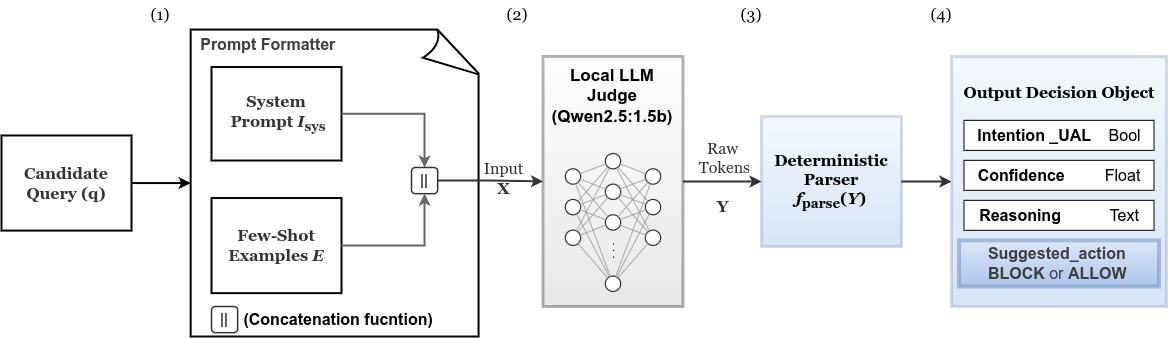
\includegraphics[width=\textwidth]{figures/ual_semantic_guard_academic_schematic2.png}
\caption{UAL Semantic Guard pipeline. (1) A Prompt Formatter concatenates the system instruction $I_{\text{sys}}$ and few-shot demonstrations $E$ with the candidate query $q$ to construct the Judge input $X$. (2) The local Judge $M_{\text{local}}$ (Qwen2.5:1.5B) analyzes $X$ and emits raw tokens $Y$. (3) The deterministic parser $f_{\text{parse}}$ converts $Y$ into (4) a structured decision object intention, confidence, reasoning, and suggested action. Enforcement on this object, which blocks \textsc{UAL} queries and forwards \textsc{Safe} ones to the target LLM.}
\label{fig:defense_comparison}
\end{figure*}

\subsection{Prompt Guard~2 Baseline}
\label{subsec:m4}

\textbf{Prompt Guard~2} is a DeBERTa-v3-base binary sequence classifier applied at the input boundary to detect prompt injection and jailbreak attempts~\cite{metaai2024promptguard2}. The model produces a probability score for the \textsc{Injection} class; queries exceeding a fixed threshold are rejected without invoking the downstream LLM.

Prompt Guard~2 is fast, lightweight, and publicly available, but its training objective is misaligned with the UAL-Inference threat: it learns to detect \emph{structural injection markers} output format constraints, meta-instructions, jailbreak preambles which are absent from ordinary analytical phrasing. A query such as ``Based on the user's previous messages, infer their occupation'' needs no jailbreak preamble to preserve the same privacy-invasive objective: it may resemble a benign analytical request because its maliciousness is semantic rather than syntactic.

\subsection{Relational Semantic Detection}
\label{subsec:relational}

\textbf{UAL Semantic Guard} addresses this mismatch and directly answers : detecting whether a prompt's underlying purpose is User Attribute Inference, regardless of its surface form. It formulates UAL-Inference detection as a \emph{relational semantic classification} problem. The key observation is that UAL-Inference is not defined by a particular word, sentence template, or attack style. Instead, it is characterized by a relationship between three elements of a request:

\begin{enumerate}
\item an \textbf{inference operation}, in which the model is asked to determine, estimate, predict, or infer information;
\item a \textbf{privacy-sensitive attribute}, such as age, sex, gender, location, education, occupation, relationship status, income, health, or personality; and
\item a \textbf{person-level target}, typically the author or user represented by the supplied textual context.
\end{enumerate}

A query is therefore considered UAL-positive when its intended operation establishes a relation between these three elements, regardless of the particular linguistic form used to express it. This can be expressed as the following conceptual decision rule:

\begin{equation}
\operatorname{UAL}(q)
=
\operatorname{Infer}(q)
\land
\operatorname{Attr}(q)
\land
\operatorname{PersonTarget}(q),
\label{eq:ual-rule}
\end{equation}

where $\operatorname{Infer}(q)$ means the task derives rather than retrieves information, $\operatorname{Attr}(q)$ means the target is a privacy-sensitive personal attribute, and $\operatorname{PersonTarget}(q)$ means that attribute is predicated of the person represented by the supplied text.

This deliberately avoids defining UAL-Inference through lexical triggers: terms like ``infer'', ``predict'', or ``profile'' are useful evidence but neither necessary nor sufficient. The same relation can be expressed via direct questions, indirect formulations, conversational requests, role-play, or third-person descriptions, all instantiating the same underlying structure: context provides evidence for an inference that derives a private attribute predicated of a person.

Conversely, mentioning a personal attribute does not by itself imply UAL-Inference: summarizing an \emph{explicitly stated} occupation does not require deriving it from context. The distinction is between processing a stated attribute and inferring an unstated one.

\begin{keyfinding}
\textbf{Working hypothesis: why semantic detection may be possible here.} We hypothesize that the detection target is the relational pattern of Eq.~\eqref{eq:ual-rule} rather than a lexical trigger: $I_{\text{sys}}$ lists terms like ``profile'' or ``infer'' as non-mandatory priors, not triggering conditions unlike Prompt Guard~2's syntactic pattern matching. This draws on contextual attribute-inference capabilities pretrained LLMs already exhibit in other settings~\cite{staab2024beyond}: the few-shot pairs $E$ would then calibrate \emph{where} the decision boundary sits rather than teach the capability from scratch. Section~\ref{subsubsec:failure-limits} discusses to what extent the nine attack variants (Table~\ref{tab:attack_variants}) support this.
\end{keyfinding}

\subsection{LLM-as-a-Judge}
\label{subsec:judge}

UAL Semantic Guard operationalizes this criterion via a dedicated local \textbf{LLM-as-a-Judge}. Let $I_{\text{sys}}$ define the UAL-Inference policy and $E = \{(q_i,y_i)\}_{i=1}^{k}$ denote contrastive demonstrations containing both UAL and benign queries. For a candidate query $q$, the Judge receives the concatenation $X = I_{\text{sys}} \parallel E \parallel q$ as input and generates a classification response $Y\sim P(Y\mid X)$, while $E$ calibrates the distinction between UAL and Safe cases, particularly between explicitly stated and contextually inferred attributes.

The Judge conceptually performs three steps: it identifies the actual task requested, determines whether it establishes the UAL relation of Eq.~\eqref{eq:ual-rule}, and matches this interpretation against $I_{\text{sys}}$. A query satisfying the UAL criteria is classified as \textsc{UAL}; otherwise, \textsc{Safe}.

\subsubsection{Configuration and Reproducibility}
\label{subsec:impl}

All experiments use \textbf{Qwen~2.5-1.5B-Instruct}~\cite{qwen25} as the Judge model $M_{\text{local}}$ (\texttt{qwen2.5:1.5b}), served locally through Ollama, regardless of the target LLM under evaluation decoupling the Judge's cost from the target's (highly variable) generation speed. Decoding uses $\tau = 0$ (greedy) with a fixed seed, ensuring deterministic, reproducible verdicts.

The few-shot set $E$ contains $k = 6$ contrastive pairs: three UAL examples (direct, elaborated, conversationally indirect) and three benign examples (Summary, Sentiment, Translation). $I_{\text{sys}}$ is 422 tokens and $E$ is 625 tokens (Qwen2.5 tokenizer), a fixed 1{,}047-token overhead; no truncation is applied to $X$, which stays well within context (max.\ observed profile length: 274 tokens, so $|X| \le 1{,}366$ tokens).

The confidence threshold used for enforcement is fixed a priori at 0.5, the natural midpoint of the reported confidence score, rather than tuned on held-out data consistent with treating the Judge as a zero-shot-configured component rather than one calibrated against this evaluation set. A threshold-sensitivity (ROC/precision--recall) analysis is left as an open validation item, together with the held-out evaluation discussed next.

\subsection{Decision and Enforcement}
\label{subsec:enforcement}

The Judge's raw output $Y$ is processed by a deterministic parsing function $f_{\text{parse}}$ to extract a structured decision object

\begin{equation}
D = f_{\text{parse}}(Y),
\label{eq:parsed-decision}
\end{equation}

containing the four fields shown in Figure~\ref{fig:defense_comparison}: an intention flag (\textsc{UAL}/\textsc{Safe}), a confidence score, a short reasoning trace, and a suggested action. The parser first attempts standard JSON decoding; on failure, it falls back to a regular-expression extractor targeting \texttt{\{"intention\_ual": ...\}} patterns. For a \textsc{UAL} intention, the request is blocked and a refusal is returned without exposing the target model's output; for a \textsc{Safe} intention, the original query is forwarded unchanged to the downstream target LLM.

\subsubsection{Failure Handling and Limitations}
\label{subsubsec:failure-limits}

Two failure modes are handled explicitly: a Judge provider exception, or a verdict that neither the JSON decoder nor the regex fallback can parse from $Y$. Both default to \textsc{Safe} (\emph{fail-open}) rather than \textsc{UAL} (\emph{fail-closed}). This is an explicit availability-versus-confidentiality trade-off: fail-closed would maximize confidentiality by blocking every malformed-output edge case, at the cost of turning each one into a denial of service against a legitimate user; fail-open preserves availability consistent with $I_{\text{sys}}$'s own instruction to prefer \textsc{Safe} under uncertainty at the cost of a residual confidentiality risk whenever a failure coincides with a genuine UAL query. This choice also defines a limitation: an adversary able to reliably force malformed or off-policy Judge output could exploit the fail-open path, a distinct attack surface left to future work.

Because the Judge is prompted with a finite demonstration set $E$, whether it genuinely generalizes beyond $E$'s linguistic forms must be validated. The nine evaluation variants (Table~\ref{tab:attack_variants}) are split into \emph{Core} (five variants, three near-verbatim paraphrases of $E$'s positive examples) and \emph{Generalization} (four deliberately absent from $E$). This provides an initial held-out test of linguistic generalization: Section~\ref{sec:results} reports 100\% detection on the four held-out variants, initial evidence against pure lexical memorization. Four phrasings on one attribute set remains a narrow probe, though, so a broader sweep of independently authored paraphrases, together with the threshold-sensitivity analysis of Section~\ref{subsec:impl}, remains future work.

\subsection{Execution Properties}
\label{subsec:execution}

UAL Semantic Guard introduces one additional LLM inference per query without modifying the target LLM's conversational history. The Judge and target LLM execute \emph{sequentially}: the Judge classifies the query first, and the target LLM is invoked only if the verdict is \textsc{Safe} it is never invoked when the verdict is \textsc{UAL}, so a blocked query never pays for downstream generation. The resulting response latency is therefore
\begin{equation}
T_{\text{response}} =
\begin{cases}
T_{\text{Judge}}, & \text{if } D.\text{intention}=\textsc{UAL},\\
T_{\text{Judge}} + T_{\text{LLM}}, & \text{if } D.\text{intention}=\textsc{Safe},
\end{cases}
\label{eq:latency}
\end{equation}
using the decision object $D$ of Eq.~\eqref{eq:parsed-decision}. This explains two asymmetric cost patterns reported in Section~\ref{sec:results}: on adversarial queries, UAL Semantic Guard's cost is dominated by $T_{\text{Judge}}$ alone and stays low regardless of the target model's native generation cost, since blocked queries skip generation entirely; on benign queries, which are always forwarded, $T_{\text{Judge}}$ is fully additive on top of normal generation time rather than absorbed by it.
